% ============= %
% Chapter: Úvod %
% Status: Final %
% ============= %

\epigraph{A~little bit of math can accomplish what all the guns and barbed wire can’t: a~little bit of math can keep a~secret.}{E. Snowden, \textit{Permanent Record}, 2019}

Jen velmi těžko si dnes dokážeme představit život ve staroorientálních říších starověké Mezopotámie. Přestože tehdejšího člověka pravděpodobně příliš netrápily otázky ochrany digitálního soukromí, počítačové bezpečnosti nebo open-source kryptografie, můžeme i~tak argumentovat, že už v~tehdejším každodenním životě v~jakési prapůvodní podobě alespoň s~jedním kryptografickým nástrojem do styku přicházel --- tím nástrojem jsou \emph{pečetě}.

Pečeť --- vynález dokonce starší než samotné \textit{písmo} --- byla dlouhá tisíciletí používána kvůli nejméně dvěma užitečným funkcím, které přímo souvisí s~moderní kryptografií. Starší z~nich je tzv.~u\-za\-ví\-ra\-cí funkce. Už ve starověku byly pečetěmi uzavírány např.\ džbány s~vínem nebo olejem, ale i~místnosti nebo domy. Praktičnost takového použití pečetí spočívala v~jeho schopnosti prokázat \emph{integritu} uzavíraného objektu --- dokud byla pečeť na džbánu s~vínem neporušená, mohli jste předpokládat, že s~obsahem džbánu nebylo manipulováno a~víno není třeba otrávené; jakmile jste do džbánu vnikli, zanechali jste nevratnou, viditelnou stopu.~\cite{sfragistika}

Druhou podstatnou funkcí pečetě byla funkce ověřovací, kterou hojně využívali panovníci a~státní aparáty. Když například sicilský král Fridrich II.\ v~roce 1212 českému králi Přemyslu Otakarovi~I.\ udělil privilegium dědičnosti jeho titulu, opatřil slavnou listinu provádějící tento akt pečetí ze zlata (neboli zlatou bulou), kterou jednoznačně zaručil její \emph{autenticitu}.~\cite{sfragistika, zlatabula}

S~rozvojem gramotnosti v~západní společnosti byly pečetě nakonec nahrazeny razítky a~vlastnoručními podpisy, které pro ověření právních dokumentů používáme dodnes. Tyto nástroje mají ale jednu nevýhodu --- nelze je dobře použít pro ověřování digitálních dat. Řešením je zcela nový ověřovací prostředek založený na asymetrické kryptografii, totiž \emph{digitální podpis}.

Všechny zmíněné prostředky pro ověřování pravosti dokumentů jsou postavené na témže předpokladu, že nemohou být (jednoduše) zfalšovány. Zatímco pečetě a~podpisy se spoléhají v~nějakém smyslu na nezfalšovatelnost fyzickou, digitální podpisy stojí zpravidla na matematickém problému, který lidstvo nedokáže bez znalosti tajného klíče efektivně vyřešit, například faktorizaci\footnote{Tj.~rozklad složeného čísla na jeho prvočíselné dělitele.} velmi velkých čísel nebo tzv.~problému diskrétního logaritmu. To z~nich činí mocný nástroj --- nezáleží na tom, kolik peněz a~technických prostředků máte, jestli jste prezident nebo diktátor; pokud neobjevíte převratný algoritmus, který by složitost daného matematického problému prolomil, podpis nezfalšujete.

Vedle integrity a~autenticity zpráv si kryptografie dává za cíl zajistit ještě jednu velmi žádanou vlastnost komunikace, kterou je její \emph{důvěrnost}. Důvěrnost zprávy jednoduše znamená její nesrozumitelnost pro neoprávněnou třetí stranu a~dosahuje se jí typicky nějakým druhem šifrování. Historická motivace pro studium šifer vychází z~vojenství --- římští císaři používali pro komunikování se svými generály jednoduché substituční šifry, notoricky známá je Caesarova šifra, která nahradí každý znak zprávy znakem, který je v~latinské abecedě o~3~místa dál (A se přepíše na D, B na E, atd.); další proslulou šifrou je Enigma, za druhé světové války používaná nacistickým Německem, k~jejímuž vyluštění přispěl stroj, který je dnes považován za předchůdce moderních počítačů. Obzvlášť v~dnešní době je ale šifrování používáno i~mimo vojenství a~diplomacii jako prostředek pro zabezpečení digitální komunikace, ochranu osobních dat, digitálního soukromí, obchodních tajemství, apod. \cite{kahn1996codebreakers}

Cílem předchozích odstavců bylo především vyzdvihnout skutečnost, že problémy, které kryptografie řeší, nejsou nikterak složité nebo nové --- nové je jen to, že místo kovových pečetí, zámků z~oceli a~strojů Enigma používáme k~utajení a~zabezpečení informací a~digitální komunikace nástroje, které nám dává algebra, teorie čísel a~další oblasti moderní matematiky. Použití matematické kryptografie pro zabezpečení informačních a~komunikačních systémů s~sebou ale kromě silných bezpečnostních záruk nese i~jednu nevýhodu: Kryptografie je složitá~\cite{youreallyshouldnt, hurdles}. Navrhnout kryptografický protokol nebo algoritmus tak, aby byl skutečně bezpečný a~poskytoval záruky, které od kryptografie očekáváme, není zdaleka jednoduché a~vyžaduje dalekosáhlou expertízu. To přirozeně vede k~jisté nerovnováze: V~době internetu a~digitální komunikace nelze potřebu kryptografie přecenit --- téměř jakákoli webová aplikace dnes musí používat kryptografické protokoly\footnote{Čtenář je jistě přinejmenším z~uživatelského hlediska obeznámen s~protokolem HTTPS, který spočívá v~obalení HTTP komunikace kryptografickým protokolem TLS.}, aby ochránila své uživatele před nemilosrdnými útočníky, kteří na internetu číhají. Takových aplikací přitom mohou být miliony~\cite{appstorestats} a~uživatelů, jejichž soukromí a~bezpečí závisí na kvalitní kryptografii, potenciálně ještě více. Oproti tomu expertů, kteří jsou takové kvalitní kryptografické algoritmy a~protokoly schopní navrhnout, je relativně málo.

V~praxi je tento problém řešen skrze standardizaci kryptografických algoritmů a~jejich otev\-ře\-nou im\-ple\-men\-ta\-ci v~\emph{kryptografických knihovnách}\footnote{Softwarová knihovna je jednoduše kód, který řeší nějakým způsobem často používanou funkcionalitu a~může být proto opětovně používán napříč programy.}.
Kryptografické algoritmy (resp.\ protokoly) na\-vr\-že\-né experty jsou podrobeny recenzi vědecké komunity a~v~případě, že se osvědčí jako bezpečné, standardizovány nějakou standardizační autoritou (např. \textit{Internet Engineering Task Force}, IETF). Zveřejněné algoritmy pak může kdokoli implementovat v~nějakém programovacím jazyce a~z\-ve\-řej\-nit je jako součást kryptografické knihovny. Aplikační vývojáři tak v~důsledku nemusí algoritmus sami programovat, ale mohou použít některou dostupnou implementaci.

Výše popsaný model není ani mimo oblast kryptografie v~softwarovém vývoji nic neobvyklého; až 96 \% dnešního softwaru nějakým způsobem na takových sdílených knihovnách závisí~\cite{synopsysossreport}. Přirozenou otázkou může --- a~mělo by --- být, kdo takové veřejně dostupné implementace tvoří a~jestli jejich autorům opravdu můžeme věřit, že je tvoří správně a~bezpečně. Relevanci takové otázky podtrhuje bezpečnostní incident z~letošního března, kdy byla nalezena zadní vrátka\footnote{Zadní vrátka, angl.\ \textit{backdoor}, je označení pro mechanismus, který výlučně jeho autorovi dovoluje později obejít bezpečnostní mechanismy daného systému.} v~populárním (až všudypřítomném) softwarovém balíčku \texttt{xz-utils}~\cite{cve-2024-3094}, která byla pravděpodobně do tohoto softwaru umístěna záměrně jedním z~jeho vývojářů.

Často slýchaný argument, který by použil dogmatický zastánce open-source kódu, tvrdí, že pokud je kód knihovny dostupný veřejně všem, pak se zákonitě najde někdo, kdo má dostatečné kompetence v~oboru informační bezpečnosti (případně i~zájem na tom, aby byl produkt bezpečný), zdrojový kód si přečte, zhodnotí jej a~případně upozorní na jeho bezpečnostní nedostatky\footnote{Ostatně \emph{v~nějakém smyslu} podobným způsobem byl objeven i~zmíněný backdoor v~\texttt{xz-utils}~\cite{vergexz}.}. S~takovým argumentem se lze ale z~pozice bezpečnostního analytika jen těžko spokojit, obzvlášť pak v~případě, že předmětem zkoumání je populární kryptografická knihovna, na jejímž kódu potenciálně závisí soukromí a~bezpečí milionů uživatelů.

Jeví se proto jako vysoce žádoucí nalézt obecnou metodu, na základě které by bylo možné s~rozumným úsilím a~nestranností zhodnotit kvalitu, bezpečnost a~důvěryhodnost dané knihovny a~rozhodnout, jestli má nebo nemá být v~projektu použita, případně pod jakými podmínkami. To je \textit{raison d'être} této práce.

\begin{figure}
    \centering
    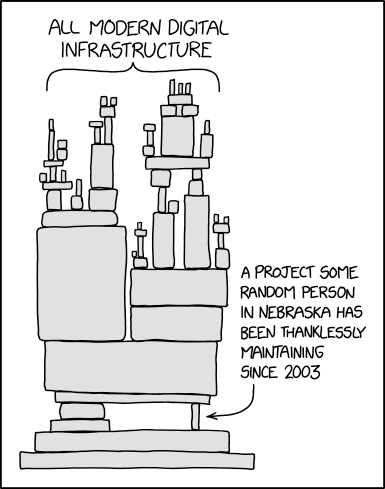
\includegraphics[width=0.5\textwidth]{text/media/dependency.png}
    \caption[~Komiks umělce xkcd s~názvem ``\textit{Dependency}'']{Komiks umělce xkcd z~roku 2020 s~názvem ``\textit{Dependency}'' ilustruje křehkost používání závislostí ve vývoji softwaru.~\cite{xkcd}}
\end{figure}

\section*{Cíle práce}\addcontentsline{toc}{section}{Cíle práce}\markboth{Cíle práce}{Cíle práce}

Jedním z~předních motivů pro vznik této práce byla účast na řešení výzkumného projektu Národního úřadu pro kybernetickou a~informační bezpečnost, který se zabýval hodnocením bezpečnosti open-source kryptografických knihoven a~identifikací rizik jejich používání --- k~řešení tohoto projektu přispívají i~bakalářské práce Matěje Douši~\cite{matej} a~Kirilla Leonova~\cite{kirill}. Cíle této práce, z~velké části kopírujíce cíle zmíněného projektu, zahrnují:

\begin{enumerate}
    
    \item provést rešerši dostupných informací o~možných způsobech hodnocení bezpečnosti open-source kryptografických knihoven, případně bezpečnosti pouze open-source knihoven, pouze kryptografických knihoven nebo softwaru obecně;

    \item navrhnout způsob, jak pro danou kryptografickou knihovnu identifikovat časté chyby nebo nepochopení, se kterými se uživatelé při práci s~ní potýkají;

    \item na základě těchto zjištění formulovat sadu kritérií, podle kterých bude s~rozumným úsilím možné zhodnotit knihovnu a~případně doporučit nebo nedoporučit její použití;

    \item na vybraných open-source kryptografických knihovnách demonstrovat získané výsledky.
    
\end{enumerate}

Potřeba takové metodiky vychází z~pozorování, že se nejeví jako proveditelné, aby každá verze každé jednotlivé knihovny implementující kryptografické algoritmy byla kompletně bezpečnostně auditována a~otestována. Zaprvé by šlo o~aktivitu tak časově, kognitivně a~ekonomicky náročnou, že by jen málokdy připadala v~úvahu, zadruhé takový postup nelze aplikovat, pokud analytik nedisponuje potřebnou expertízou. Nakonec by ani takový přístup nemusel nutně pokrýt všechny aspekty bezpečnosti knihovny, jako například pravděpodobnost, že ji i~další uživatel, který nezná detailně její vnitřní fungování, bude schopný správně použít.

Text této práce je dále organizován následujícím způsobem. Kapitoly~\ref{software} a~\ref{pouziti} uvedou čtenáře do problematiky bezpečnosti softwaru, resp.\ zranitelného použití kryptografie a~jeho předcházení, a~shrnou vědecké poznatky v~těchto oblastech. V~kapitole~\ref{analyza} popíšeme vybrané kryptografické knihovny a~provedeme analýzu jejich relevantních vlastností. Výslednou metodu pro hodnocení bezpečnosti kryptografických knihoven popíšeme v~kapitole~\ref{vysledky} a~výsledky práce shrneme v~závěrečné kapitole~\ref{zaver}.
